\chapter{Tests}
In diesem Kapitel werden die Tests näher erläutert, die während der Implementierung des Systems durchgeführt wurden.

\section{Test mit der ROS Umgebung}

Die Roboterkontrollarchitektur ROS hat für die Entwicklung verschiedene Tools zur Verfügung. Dazu können grafische und auch Befehlszeile Programme verwendet werden, um das laufende System zu Debuggen.\\
Ein grafisches Programm ist \textit{RVIZ}, das 3-D-Visualisierung von Sensordaten, Robotermodellen und anderen 3-D-Daten ermöglicht. Durch diese Software konnten Sensordaten visualisiert und somit geholfen werden, die Implementierung greifbarer zu machen. So konnte schnell entdeckt werden, dass der LiDAR Scanner bei Messungen seitlich des Roboters Probleme aufzeigt.\\
Die \textit{rqt\_graph} ist ein Tool, um die aktiven Knoten, Topics und deren Verbindung grafisch als Diagramm darzustellen. Damit konnte in der Entwicklung zur Laufzeit aufgezeigt werden, wie die einzelnen Topics miteinander kommunizieren. Bei falscher Schreibweise der Topics führt es nicht in erster Linie zum Fehler, sondern zu neuen Topics die nicht existieren. Um solche Inkorrektheit zu sehen, kann diese Software verwendet werden. So kann durch die Darstellung der Verbindungen auch auf den ersten Blick gesehen werden, welche Verbindungen nicht stimmen. \\
Weitere Werkzeuge sind die Befehlszeilen-Tools. Sie ermöglichen zur Laufzeit Informationen zu den einzelnen Knoten, Topics oder Nachrichten auszugeben. Es können Sensor-Topics ausgeben werden, die während der Laufzeit überwacht werden können. Sie bieten aber auch die Möglichkeit, Verbindungen oder die Anzahl davon abzudrucken und somit eine nicht grafische Art von \textit{rqt\_graph} darstellt. Diese Kommandozeilen Werkzeuge werden häufig verwendet, da sie eine schnelle und unkomplizierte Lösung sind.

\section{API Test mit einer grafischen Oberfläche}
Um die Schnittstelle zu testen, wurde mithilfe der firmeninternen Software eine grafische Oberfläche entwickelt. Die firmeninterne Software basiert auf \textit{Windows Presentation Foundation}, kurz \textit{WPF} Anwendung und heißt \textit{Interactive Graphic Panel}, kurz genannt \textit{IGP}. Die Software ist so aufgebaut, dass im Hintergrund eine \textit{WPF} Anwendung läuft mit vielen \textit{C\#} Funktionalitäten wie TCP oder UDP Sockets, aber die grafische Benutzeroberfläche und die Interaktivität wird mit Javascript programmiert und mithilfe von \textit{XML} werden die Layouts der einzelnen Seiten erstellt. So konnte schnell eine Mensch-Maschinen-Interaktion erstellt werden, die zu Testzwecken verwendet werden konnte (siehe \autoref{fig:GUI}). \\ 

\begin{figure}[H]
\captionsetup[subfloat]{labelformat=empty}
  \centering
  \subfloat[][]{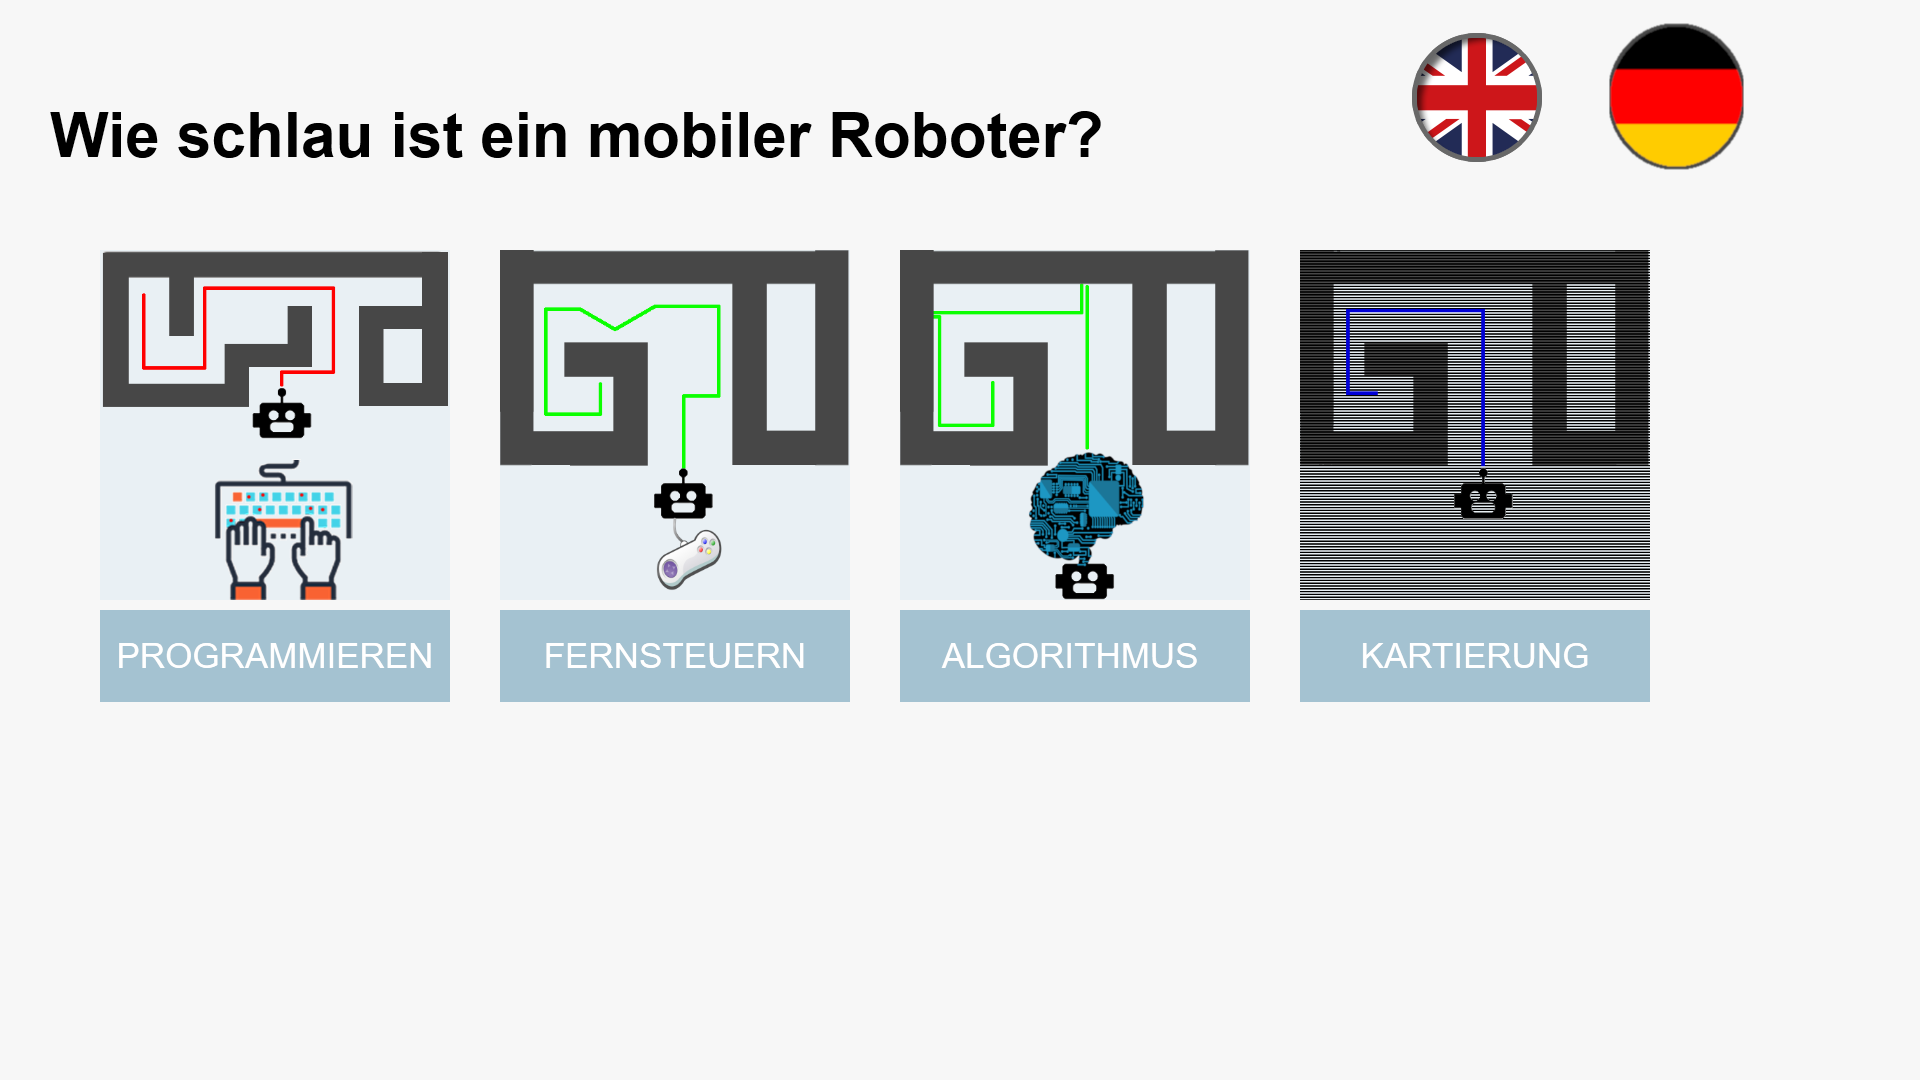
\includegraphics[width=0.5\linewidth]{Bilder/Tests/home_de.PNG}}%
  \subfloat[][]{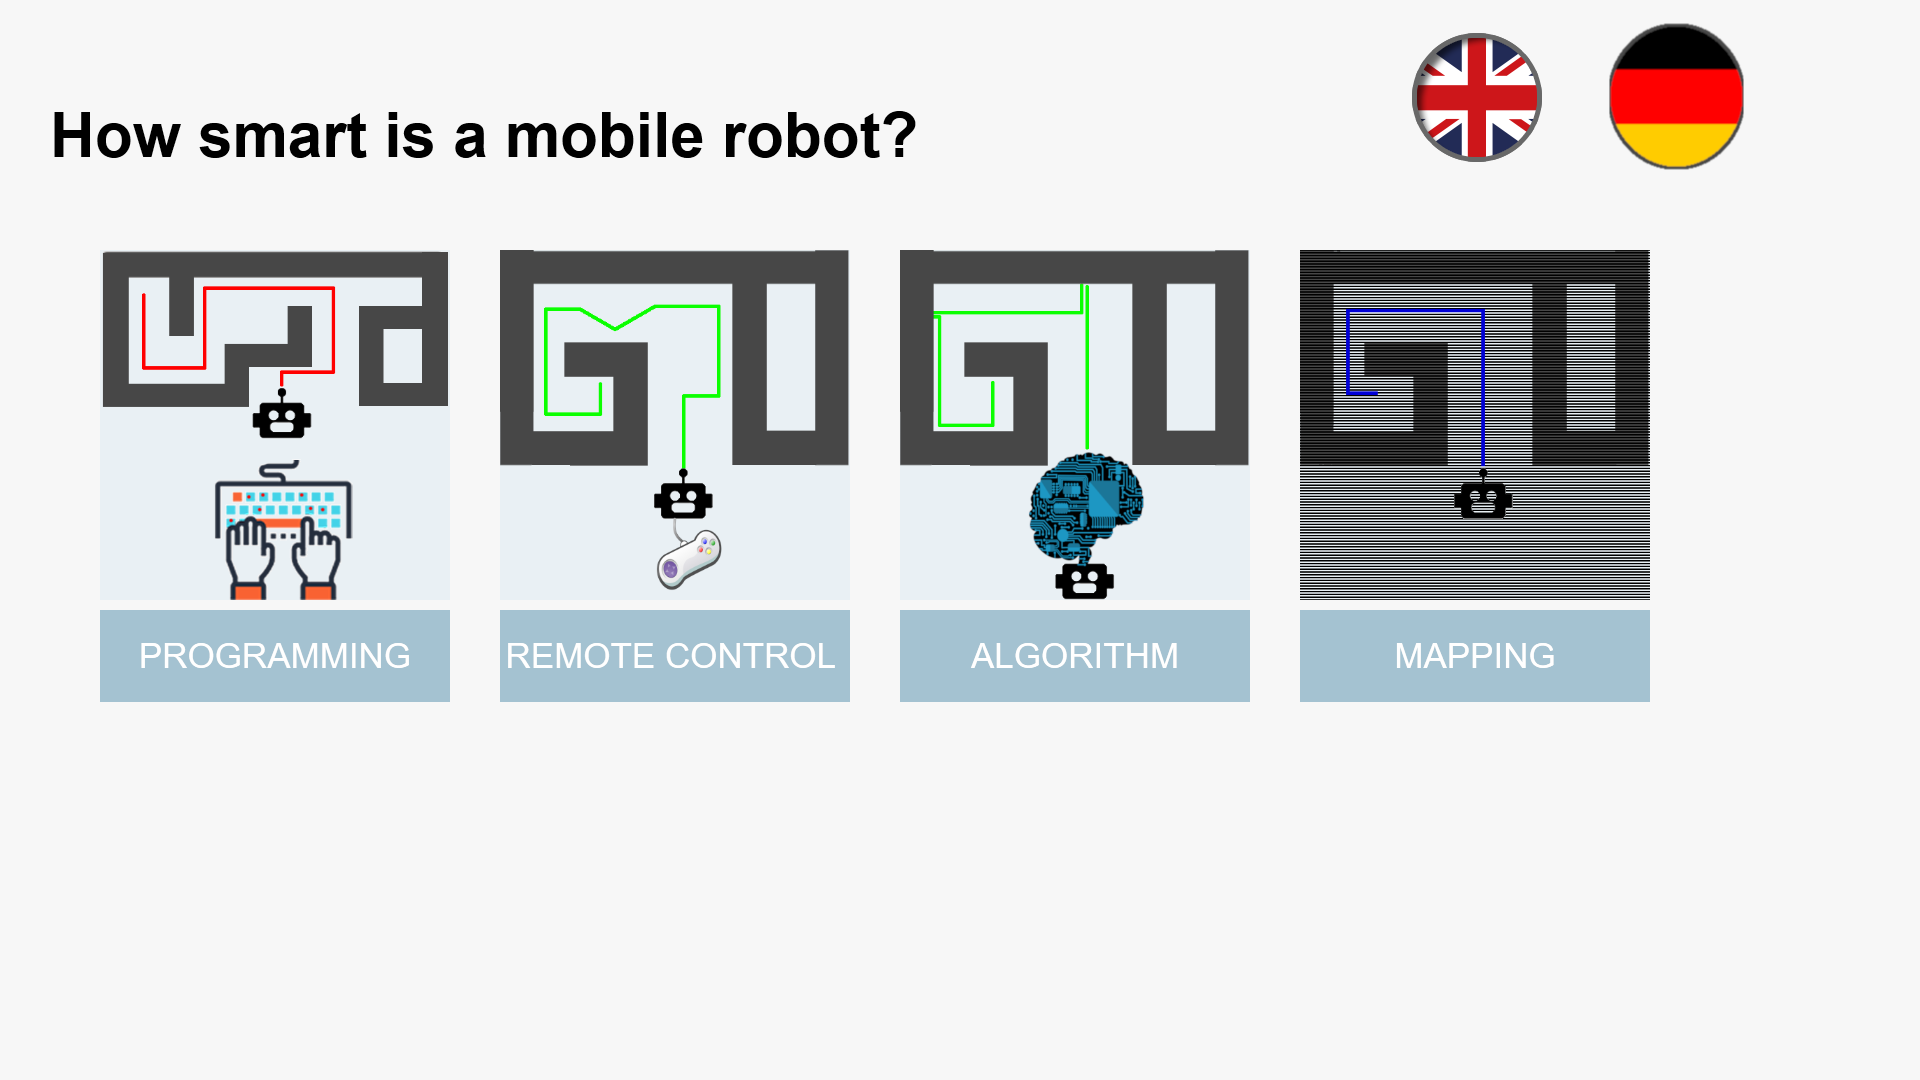
\includegraphics[width=0.5\linewidth]{Bilder/Tests/home_en.PNG}}%
  \qquad
  \subfloat[][]{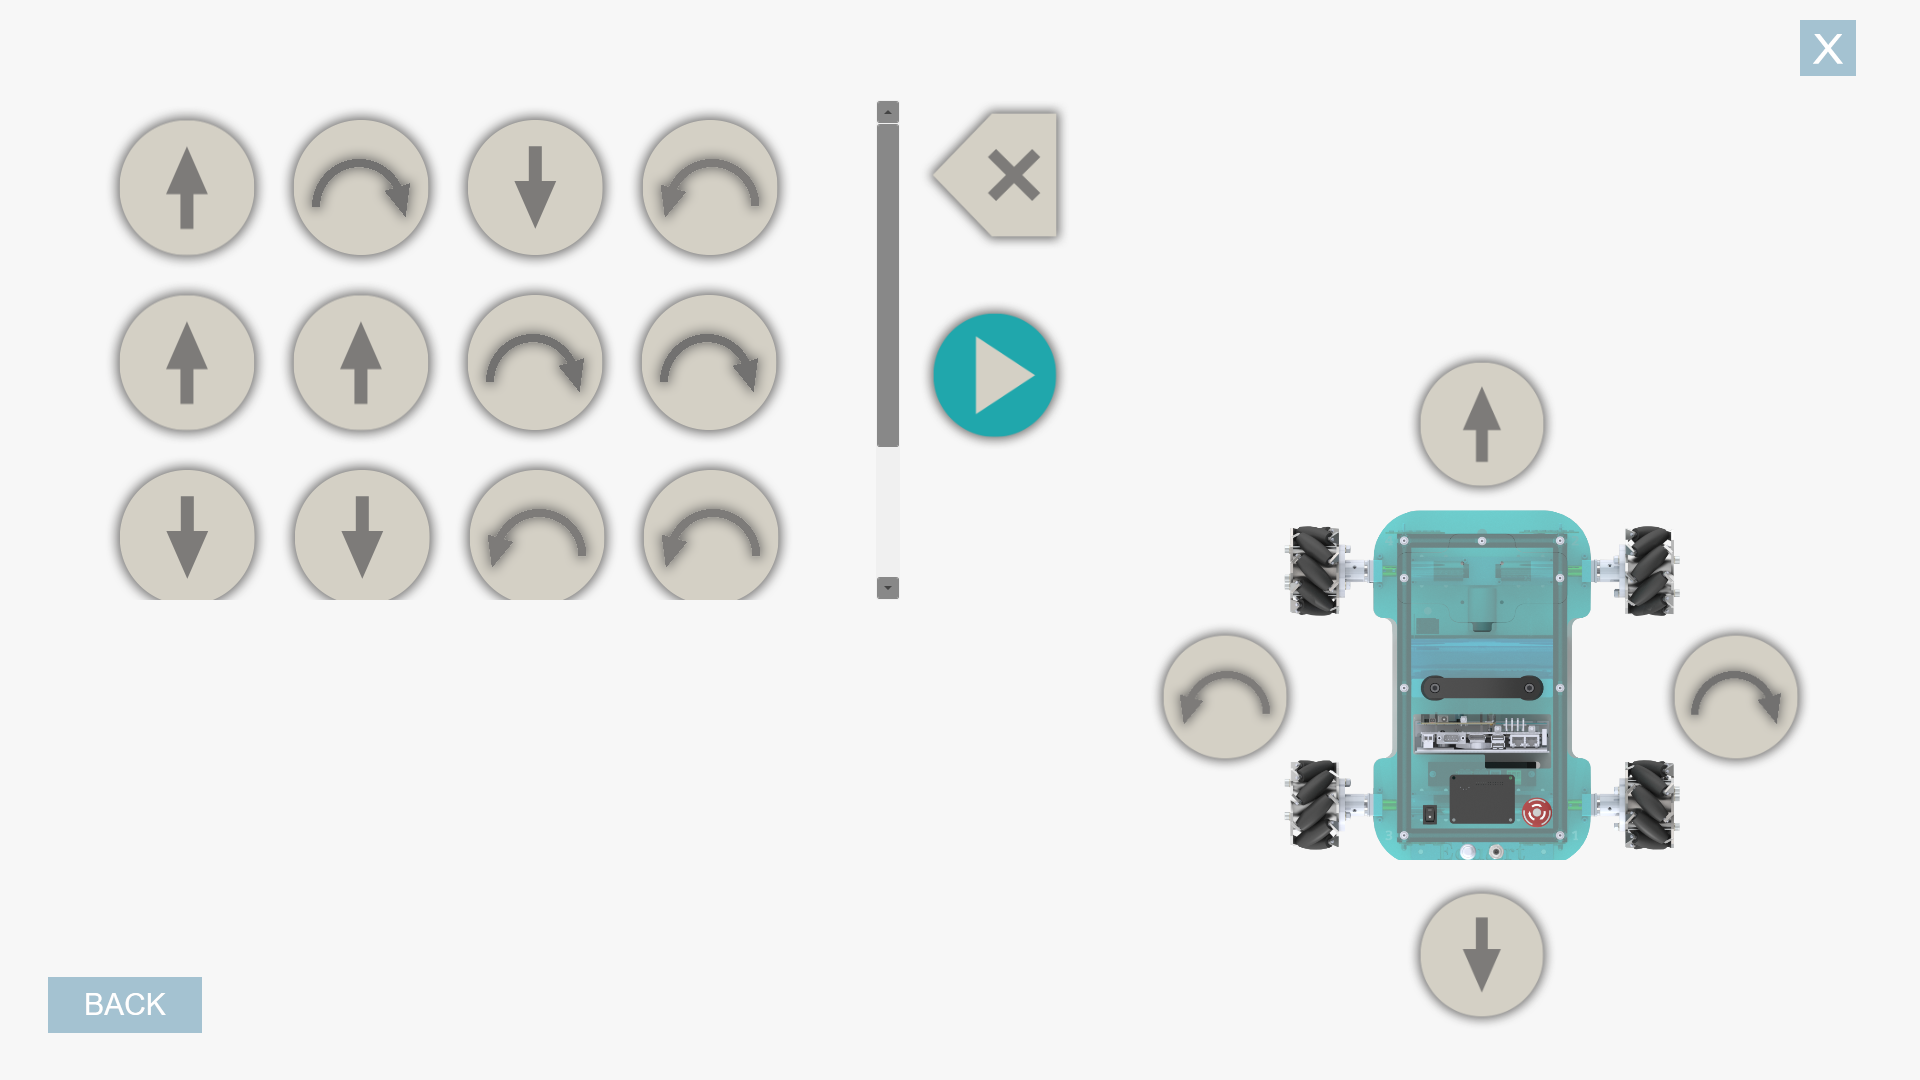
\includegraphics[width=0.5\linewidth]{Bilder/Tests/programming_scroll_scroll.PNG}}%
  \subfloat[][]{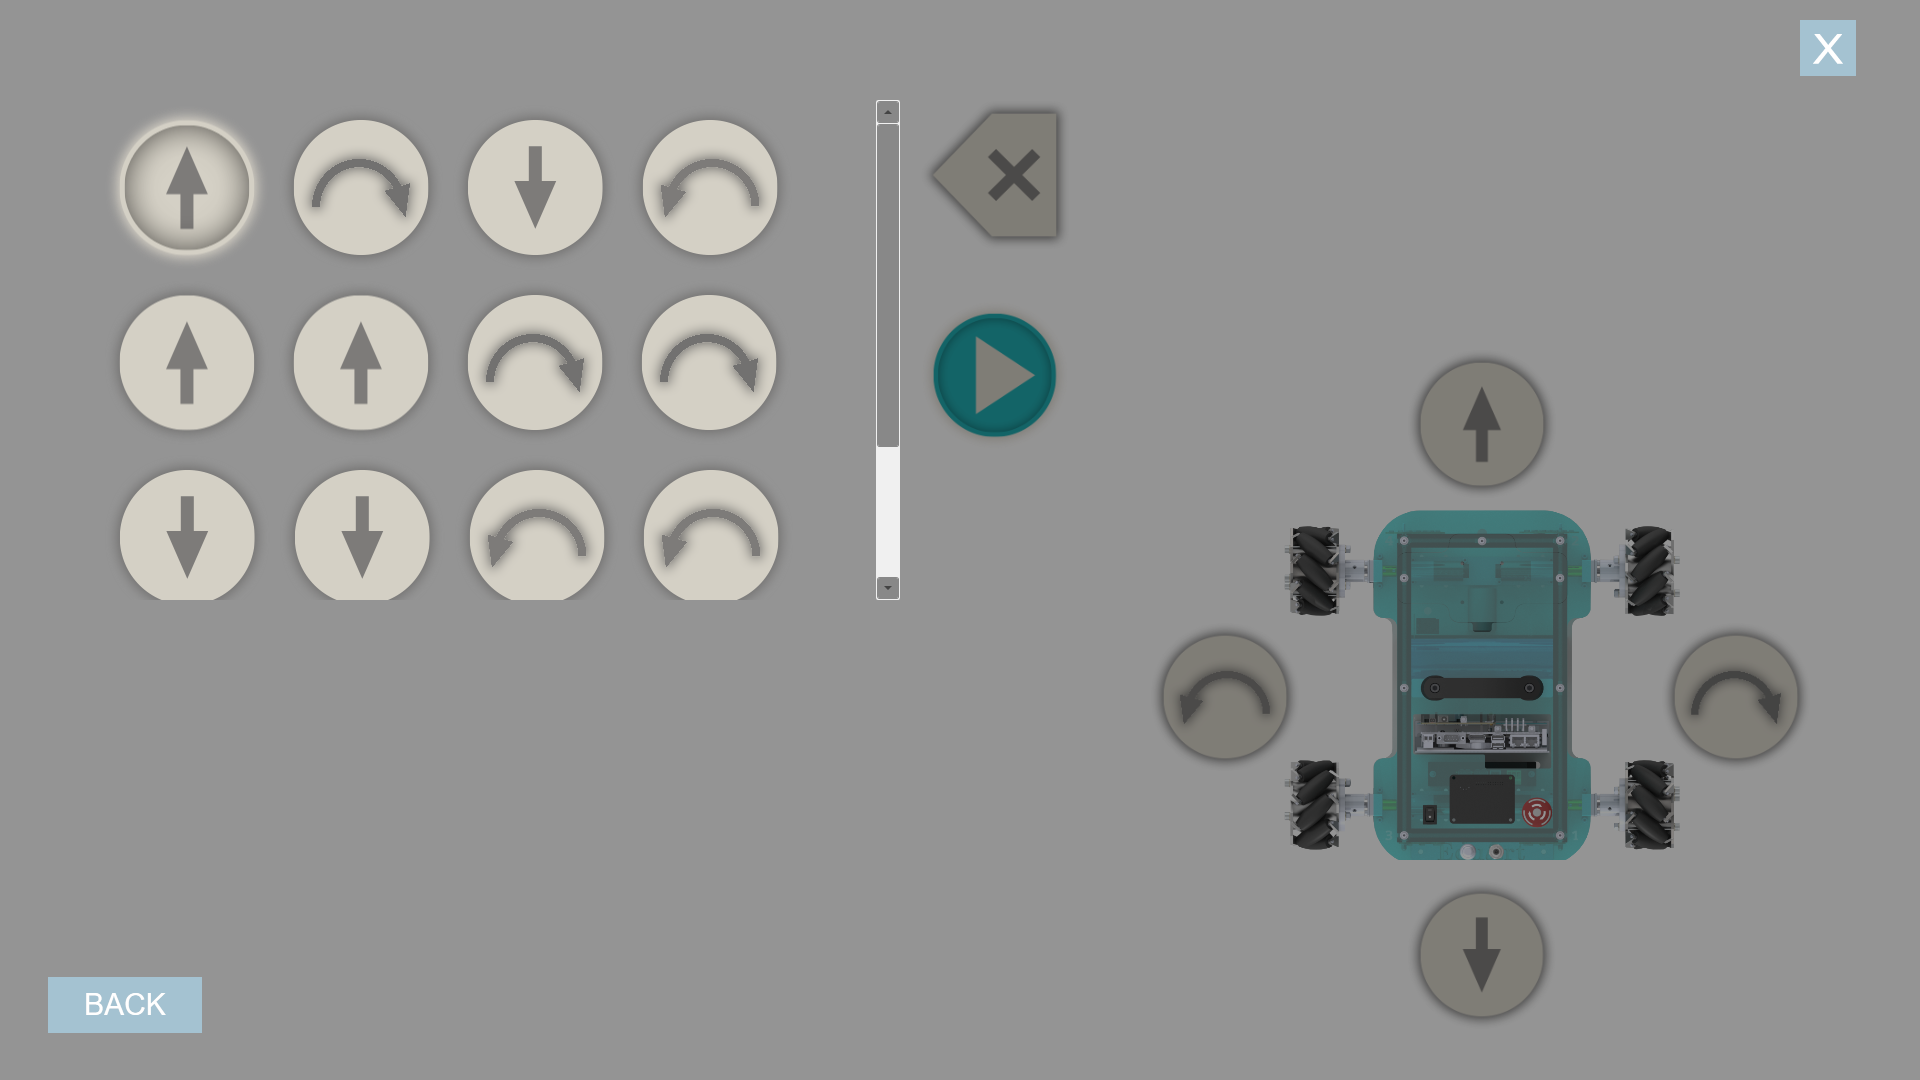
\includegraphics[width=0.5\linewidth]{Bilder/Tests/programming_aktive_scroll.PNG}}%
  \qquad
  \label{fig:GUI1}
\end{figure}

\begin{figure}[H]
\captionsetup[subfloat]{labelformat=empty}
  \centering
%   \subfloat[][]{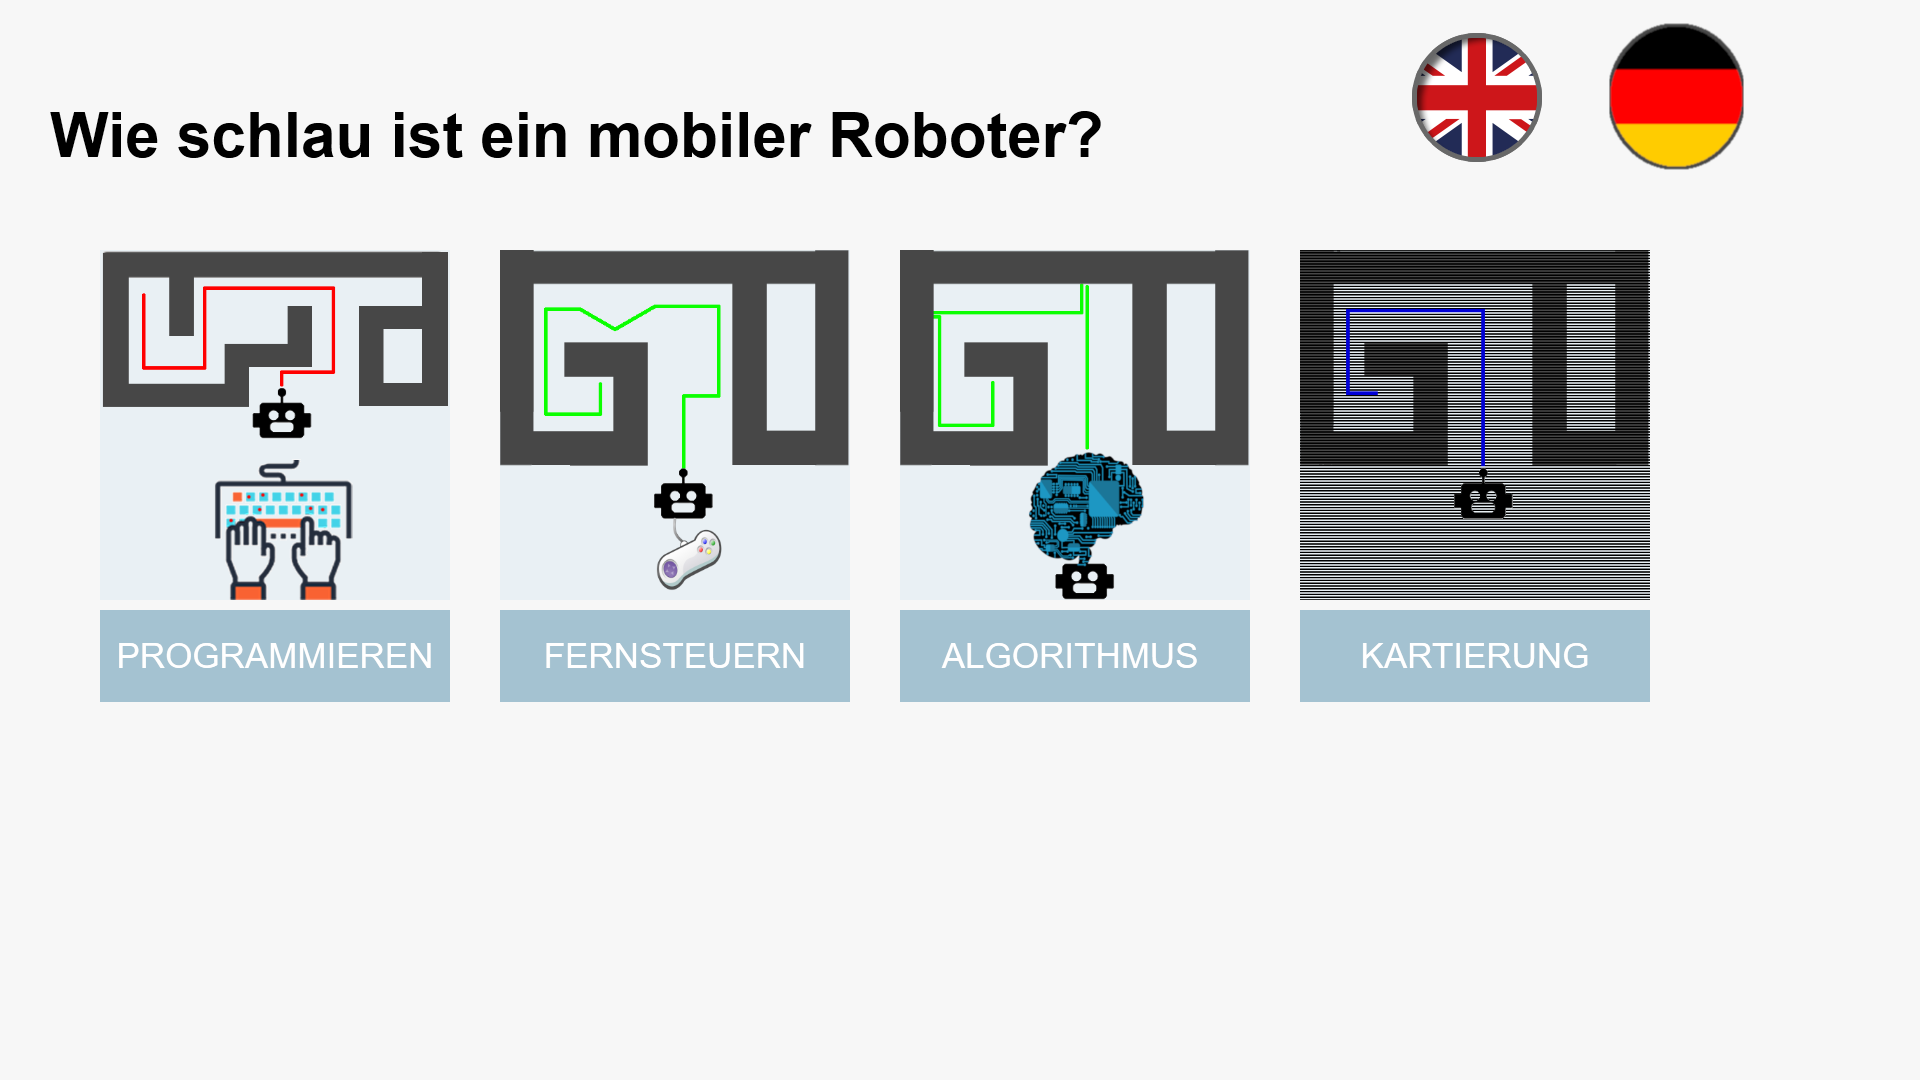
\includegraphics[width=0.5\linewidth]{Bilder/Tests/home_de.PNG}}%
%   \subfloat[][]{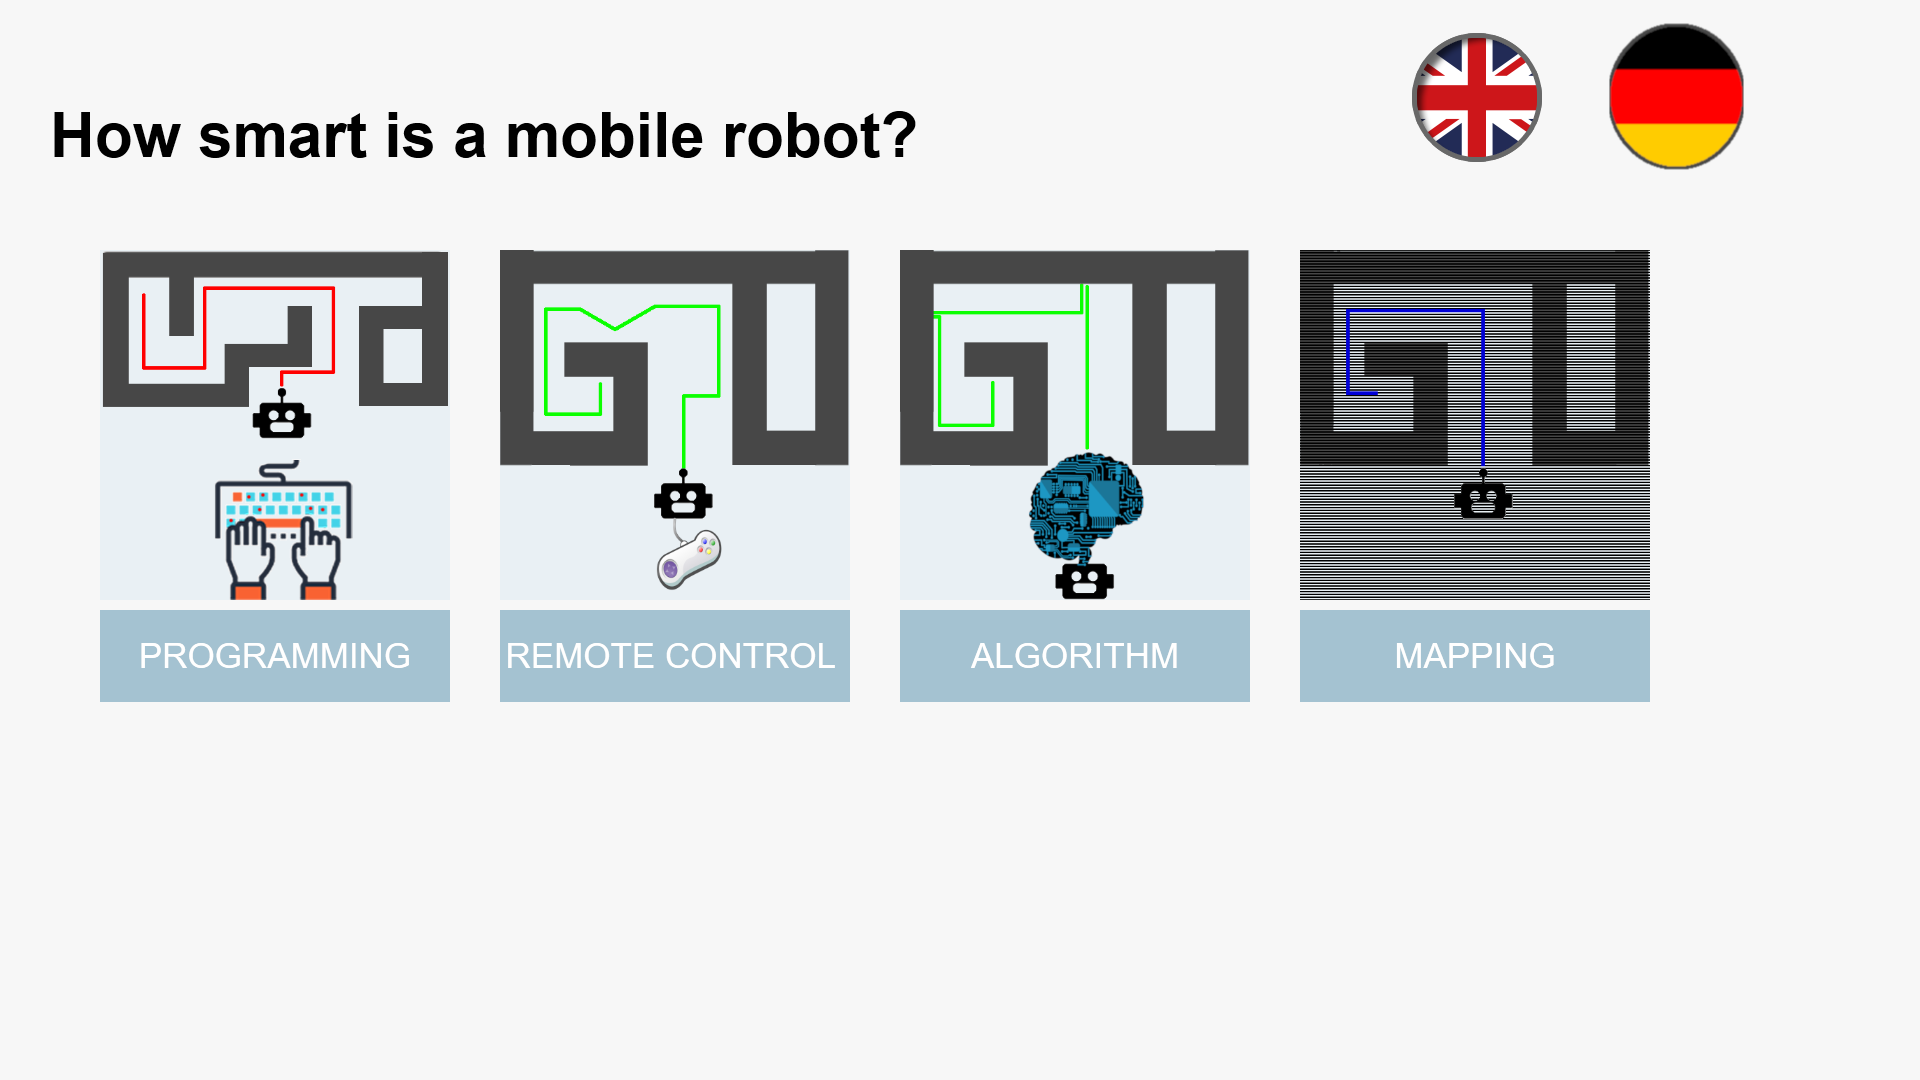
\includegraphics[width=0.5\linewidth]{Bilder/Tests/home_en.PNG}}%
%   \qquad
% %   \subfloat[][]{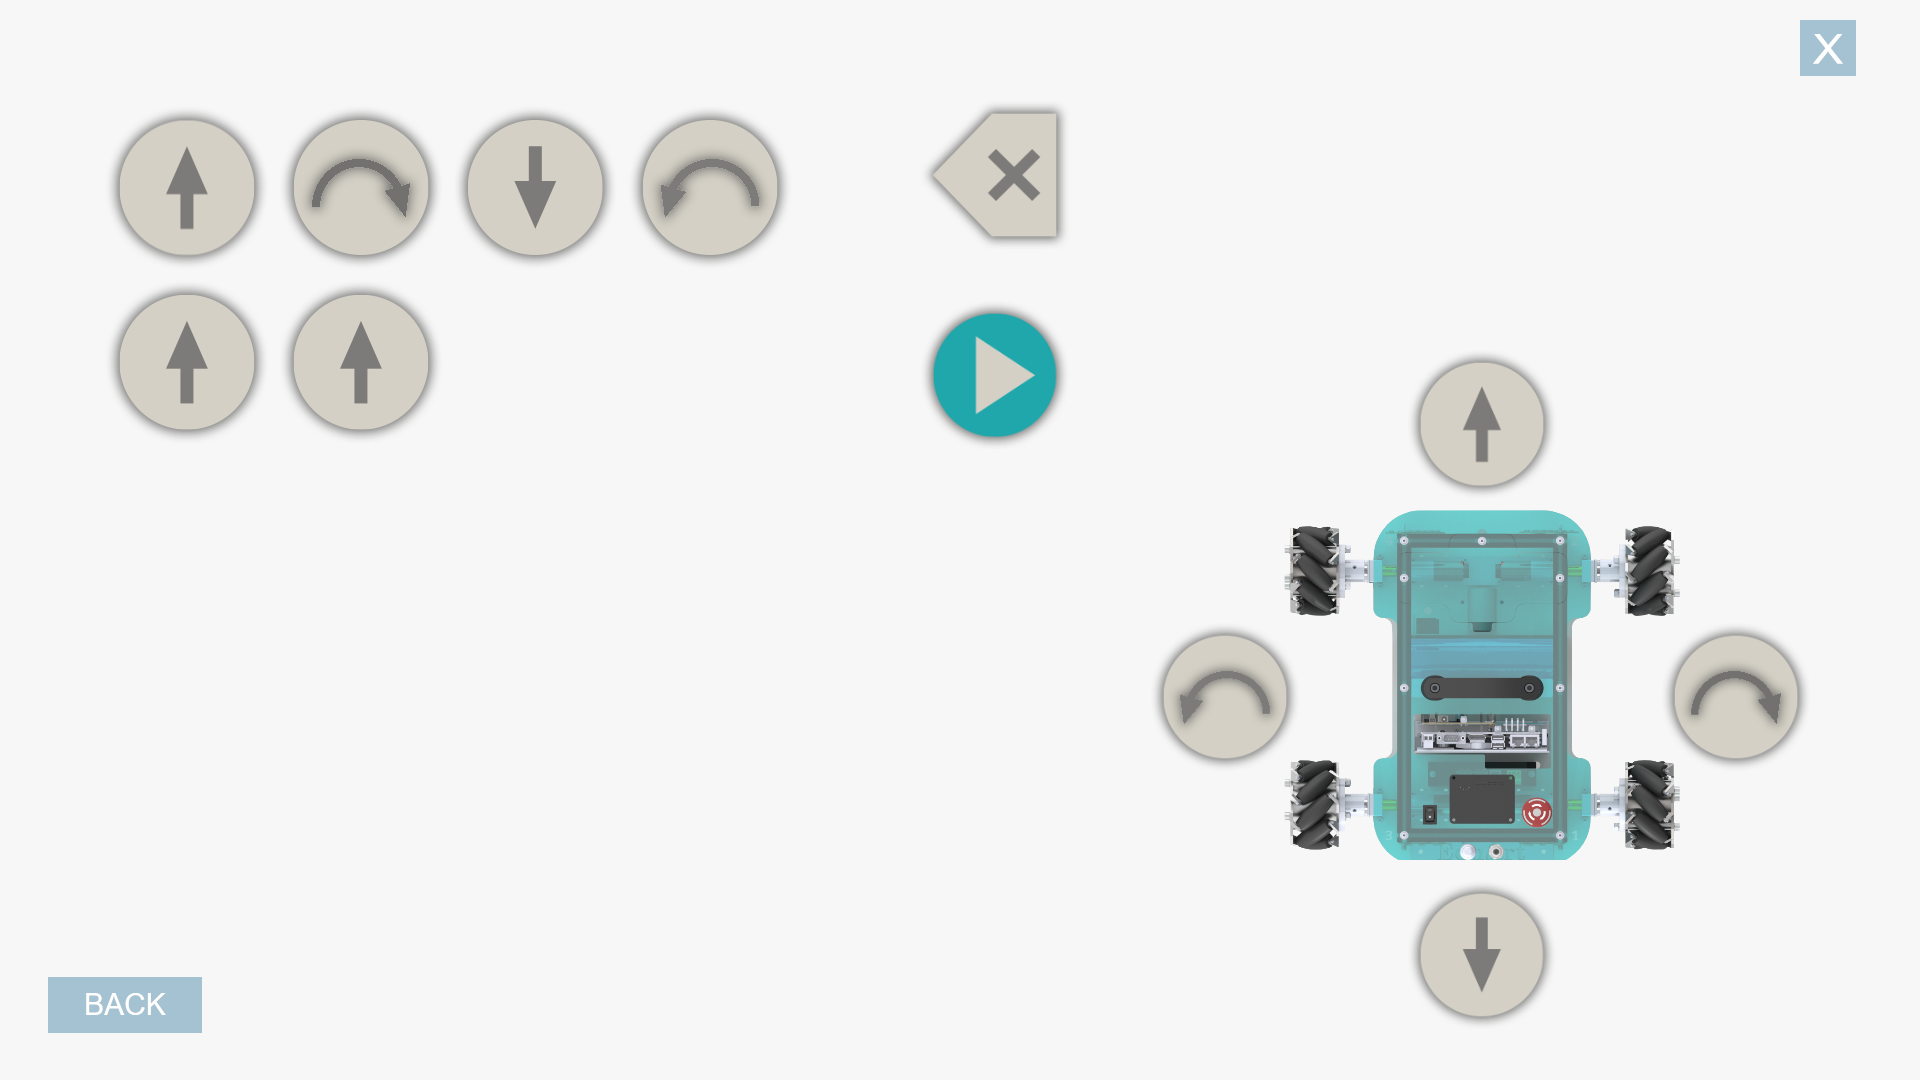
\includegraphics[width=0.5\linewidth]{Bilder/Tests/programming.PNG}}%
% %   \subfloat[][]{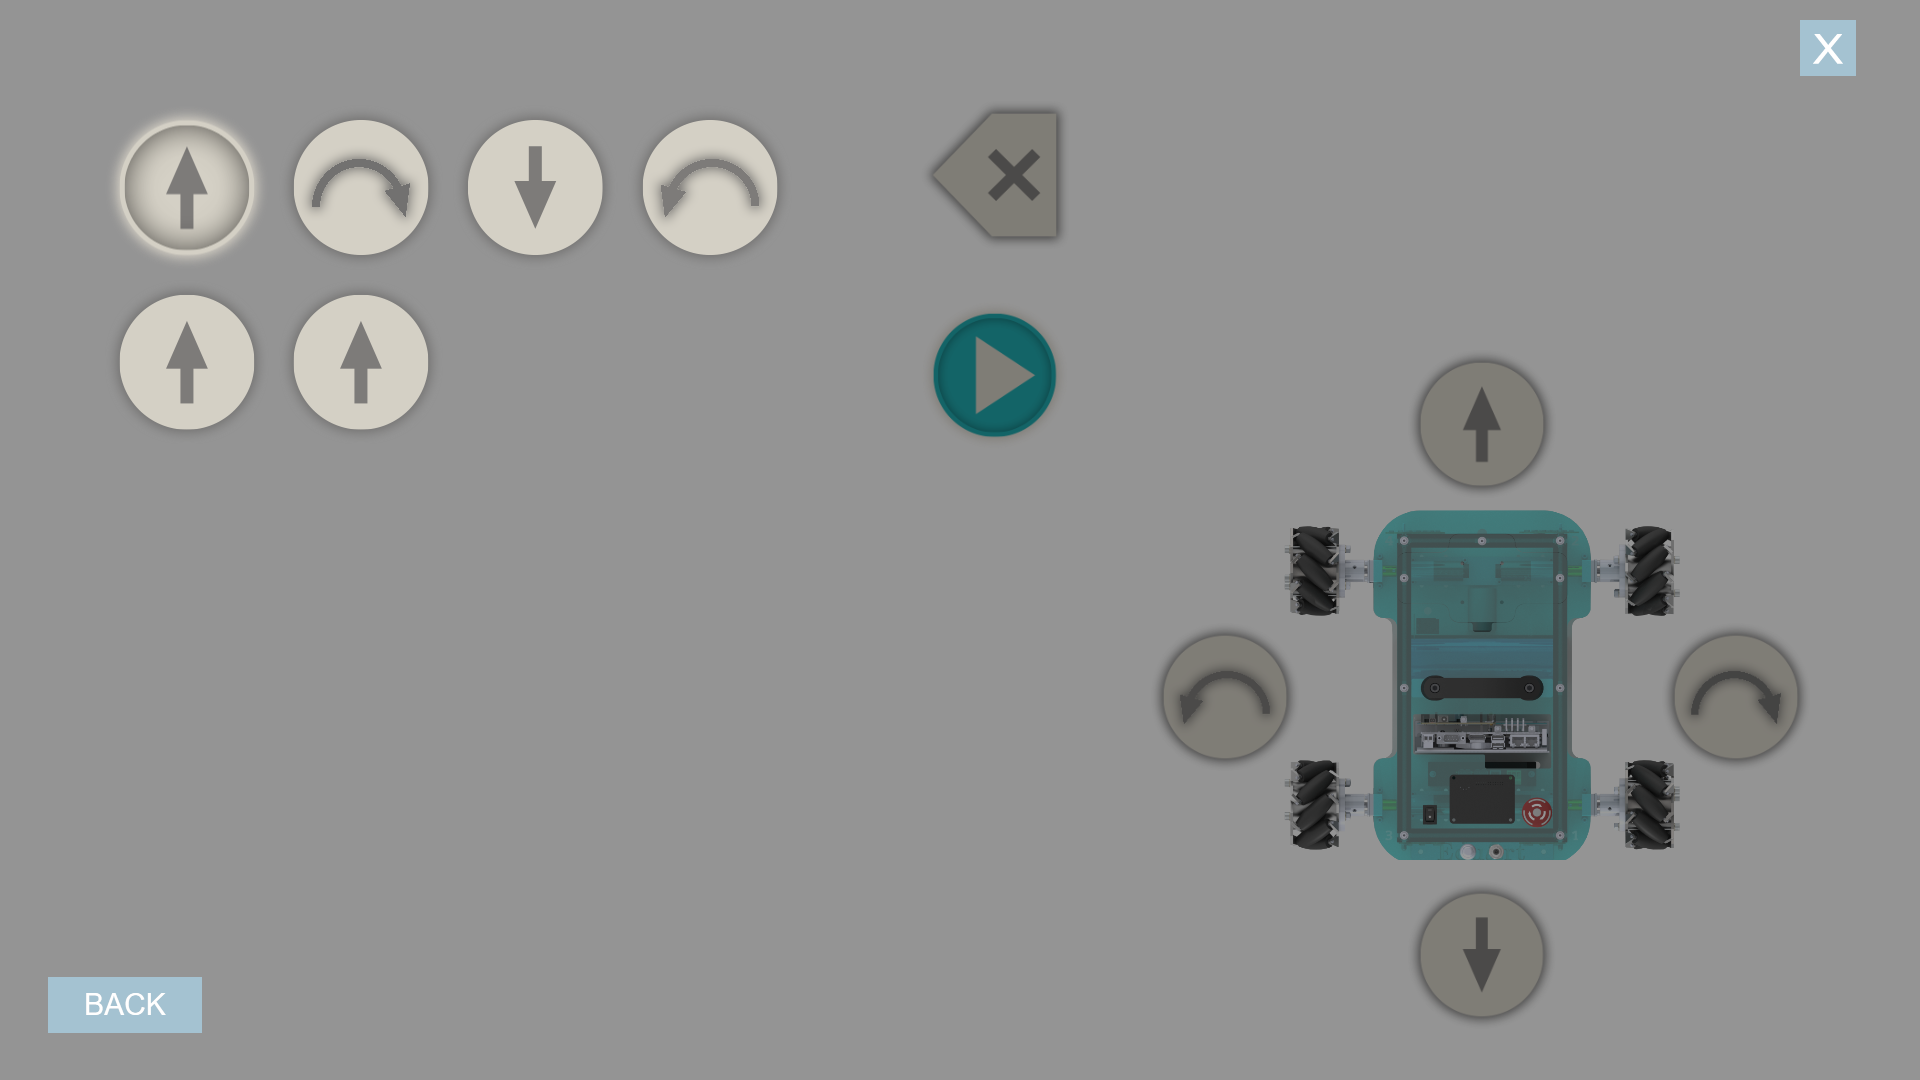
\includegraphics[width=0.5\linewidth]{Bilder/Tests/programming_aktive.PNG}}%
% %   \qquad
%   \subfloat[][]{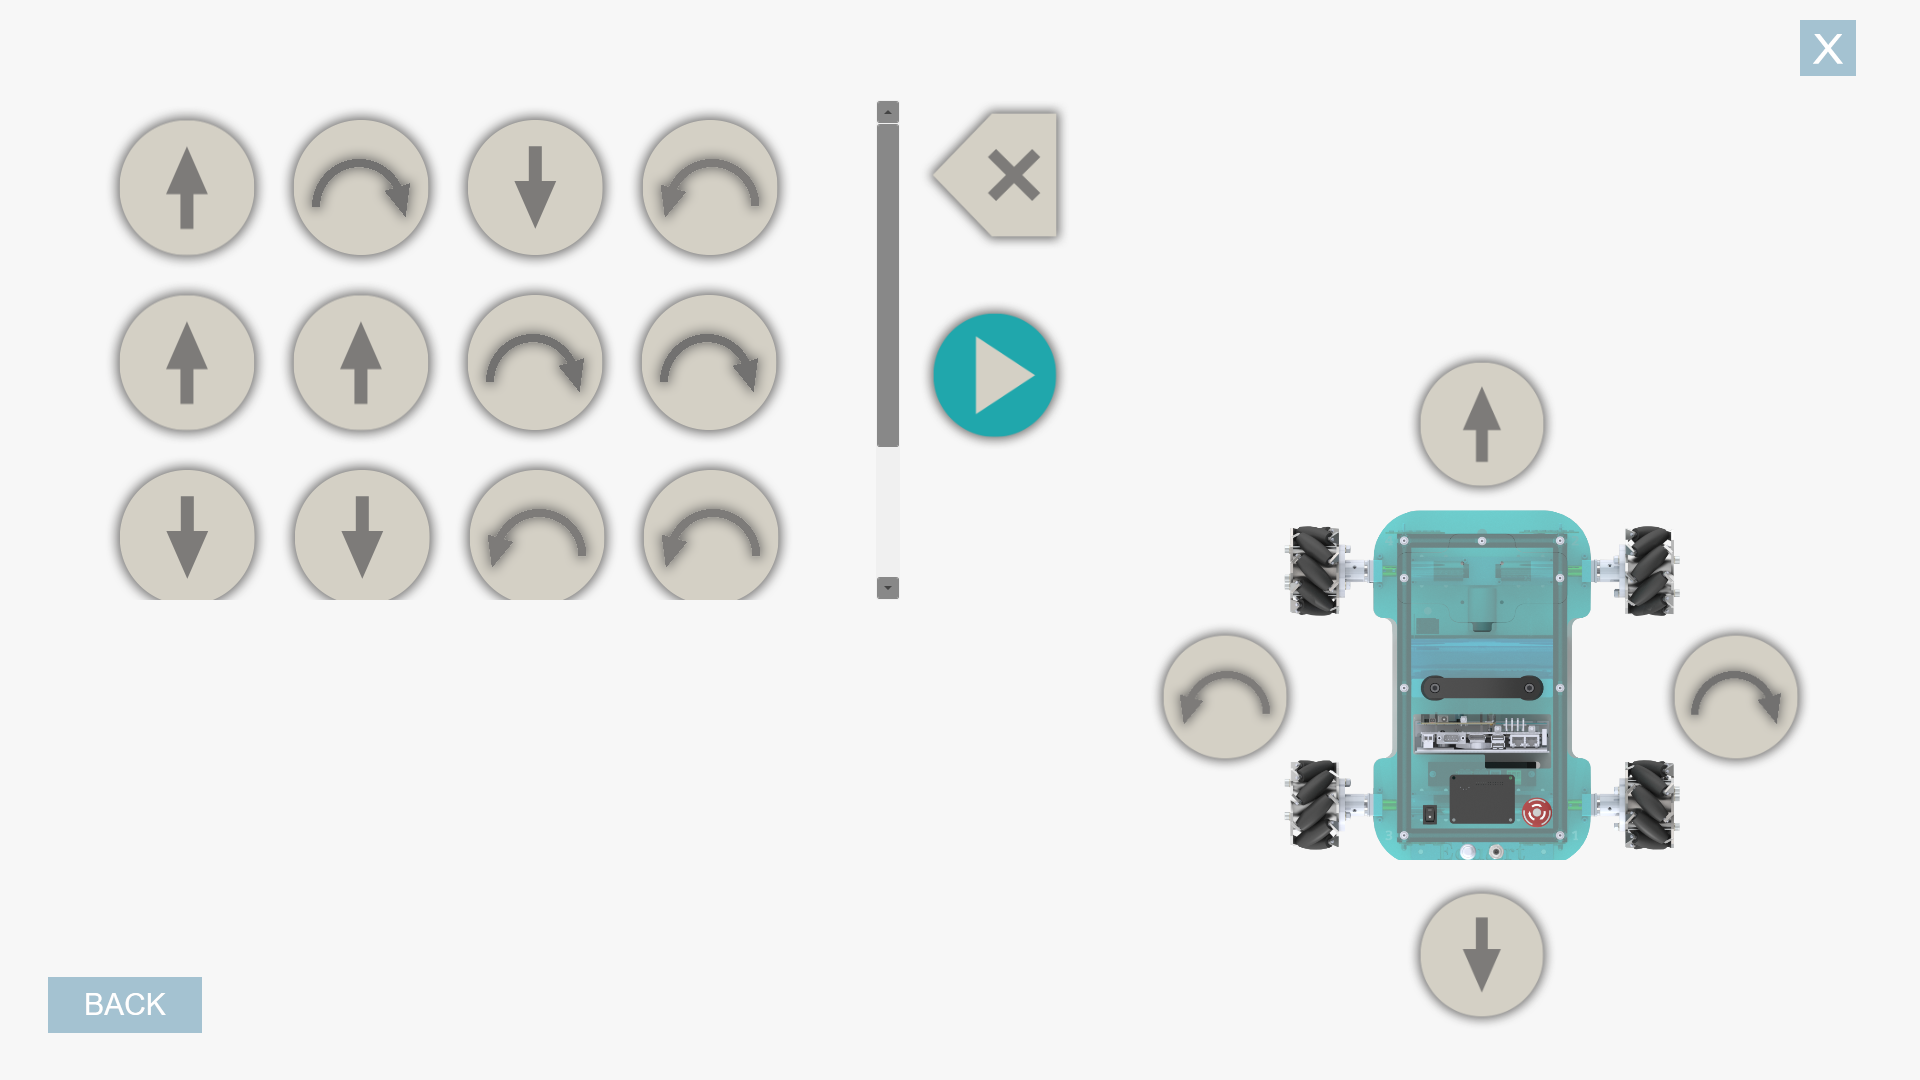
\includegraphics[width=0.5\linewidth]{Bilder/Tests/programming_scroll_scroll.PNG}}%
%   \subfloat[][]{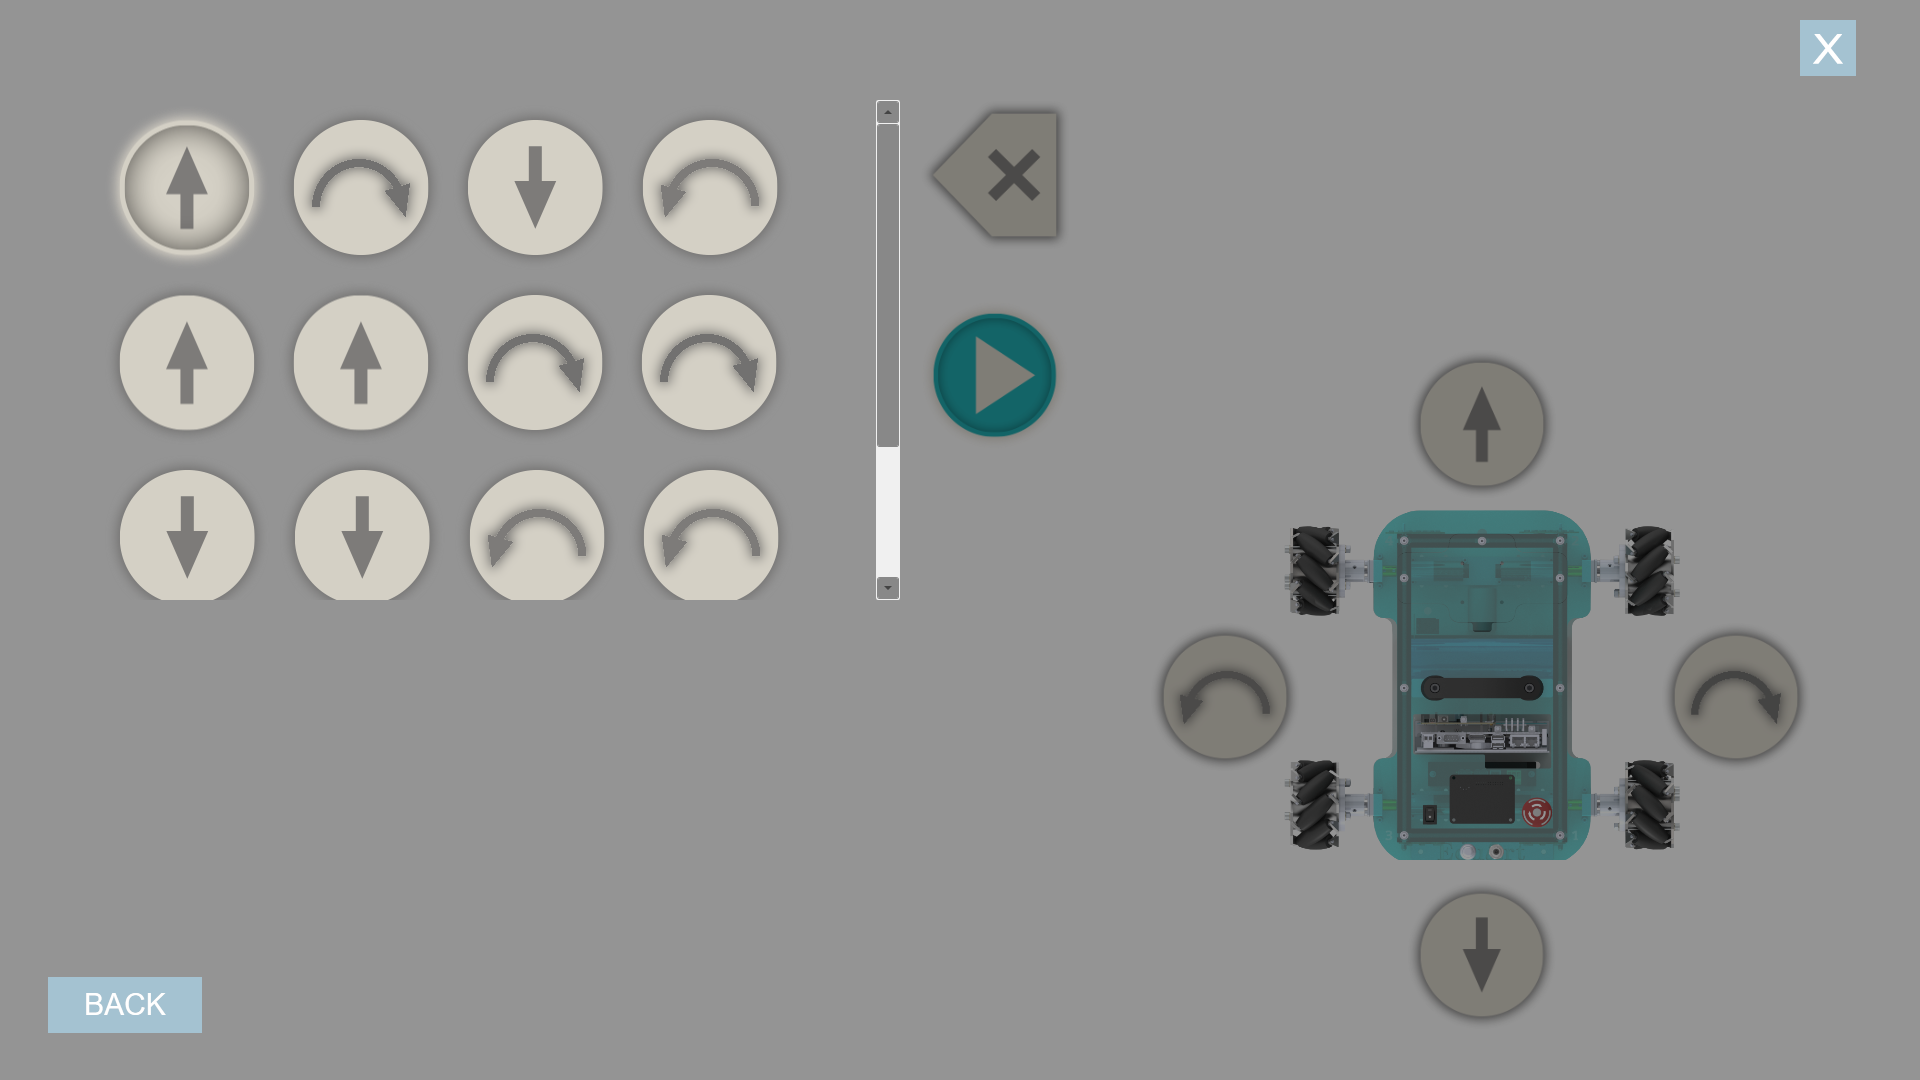
\includegraphics[width=0.5\linewidth]{Bilder/Tests/programming_aktive_scroll.PNG}}%
%   \qquad
  \subfloat[][]{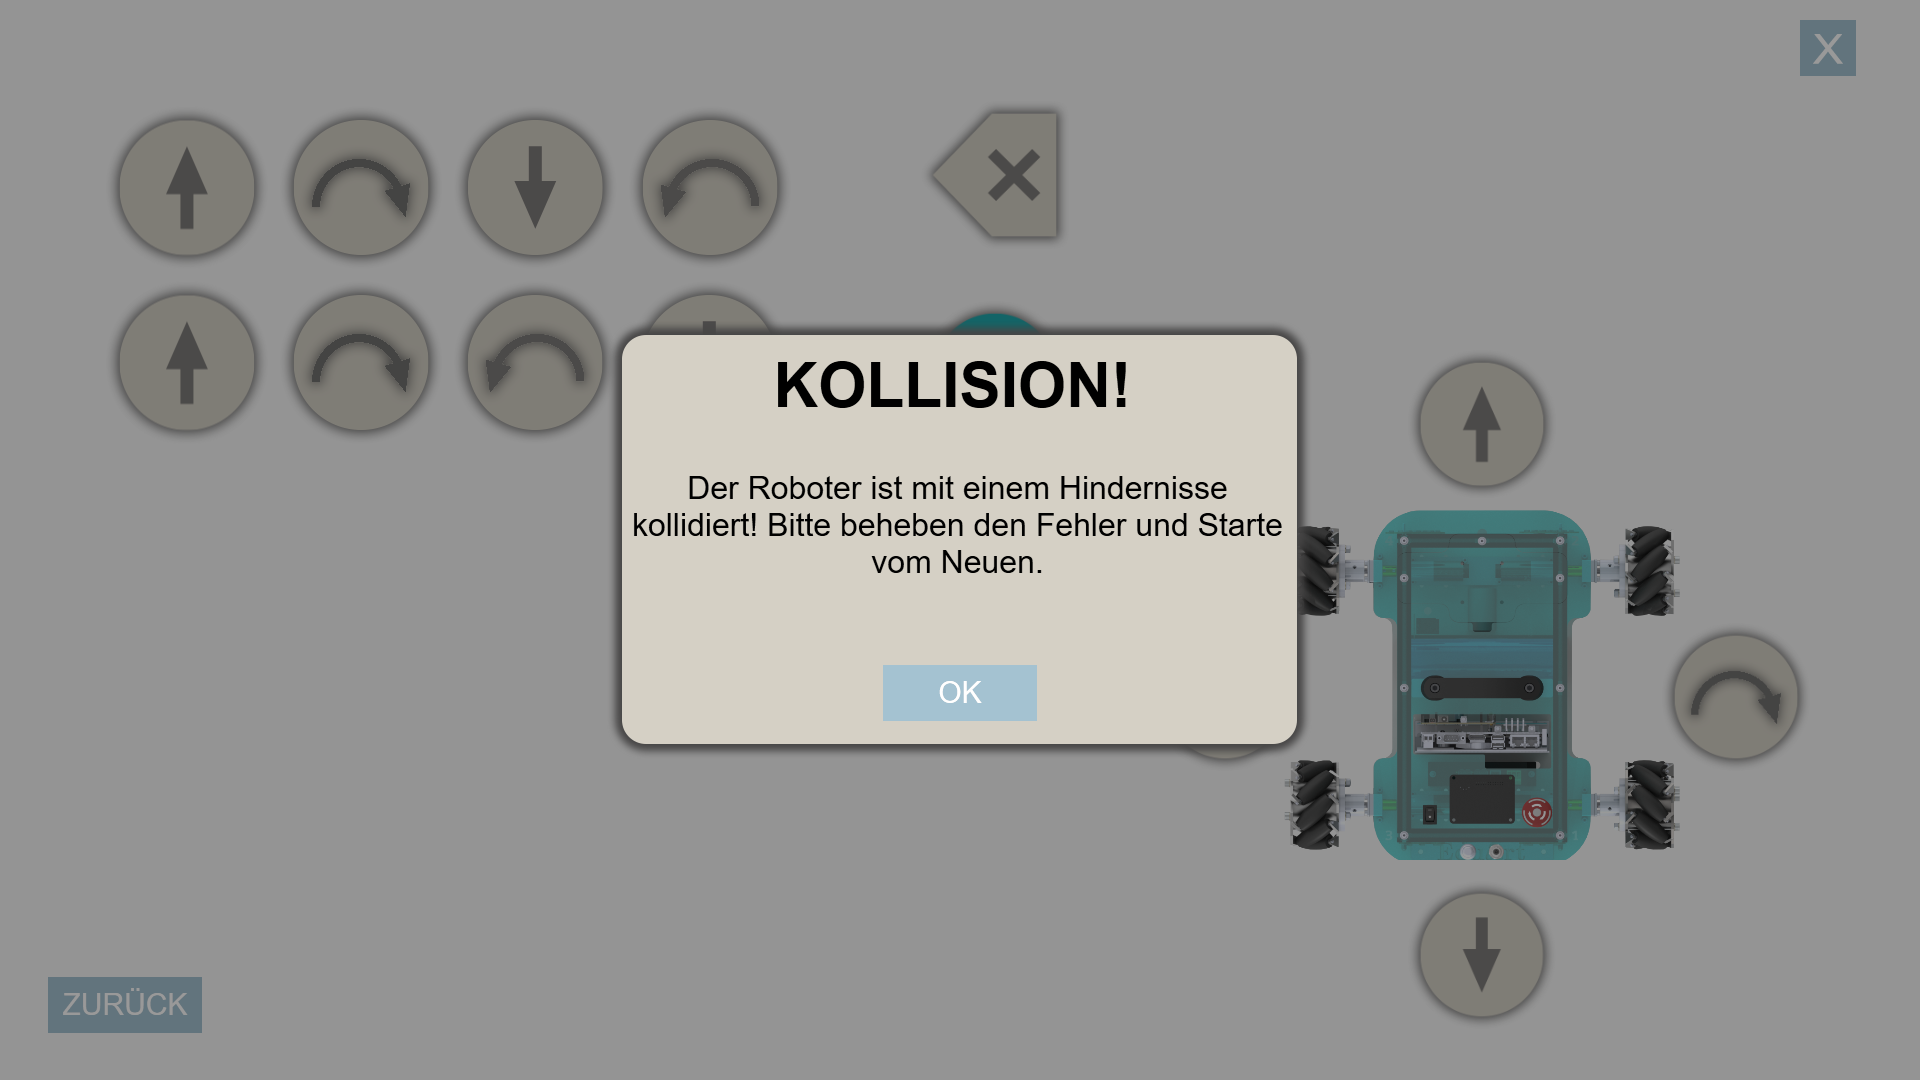
\includegraphics[width=0.5\linewidth]{Bilder/Tests/kollision_de.PNG}}%
  \subfloat[][]{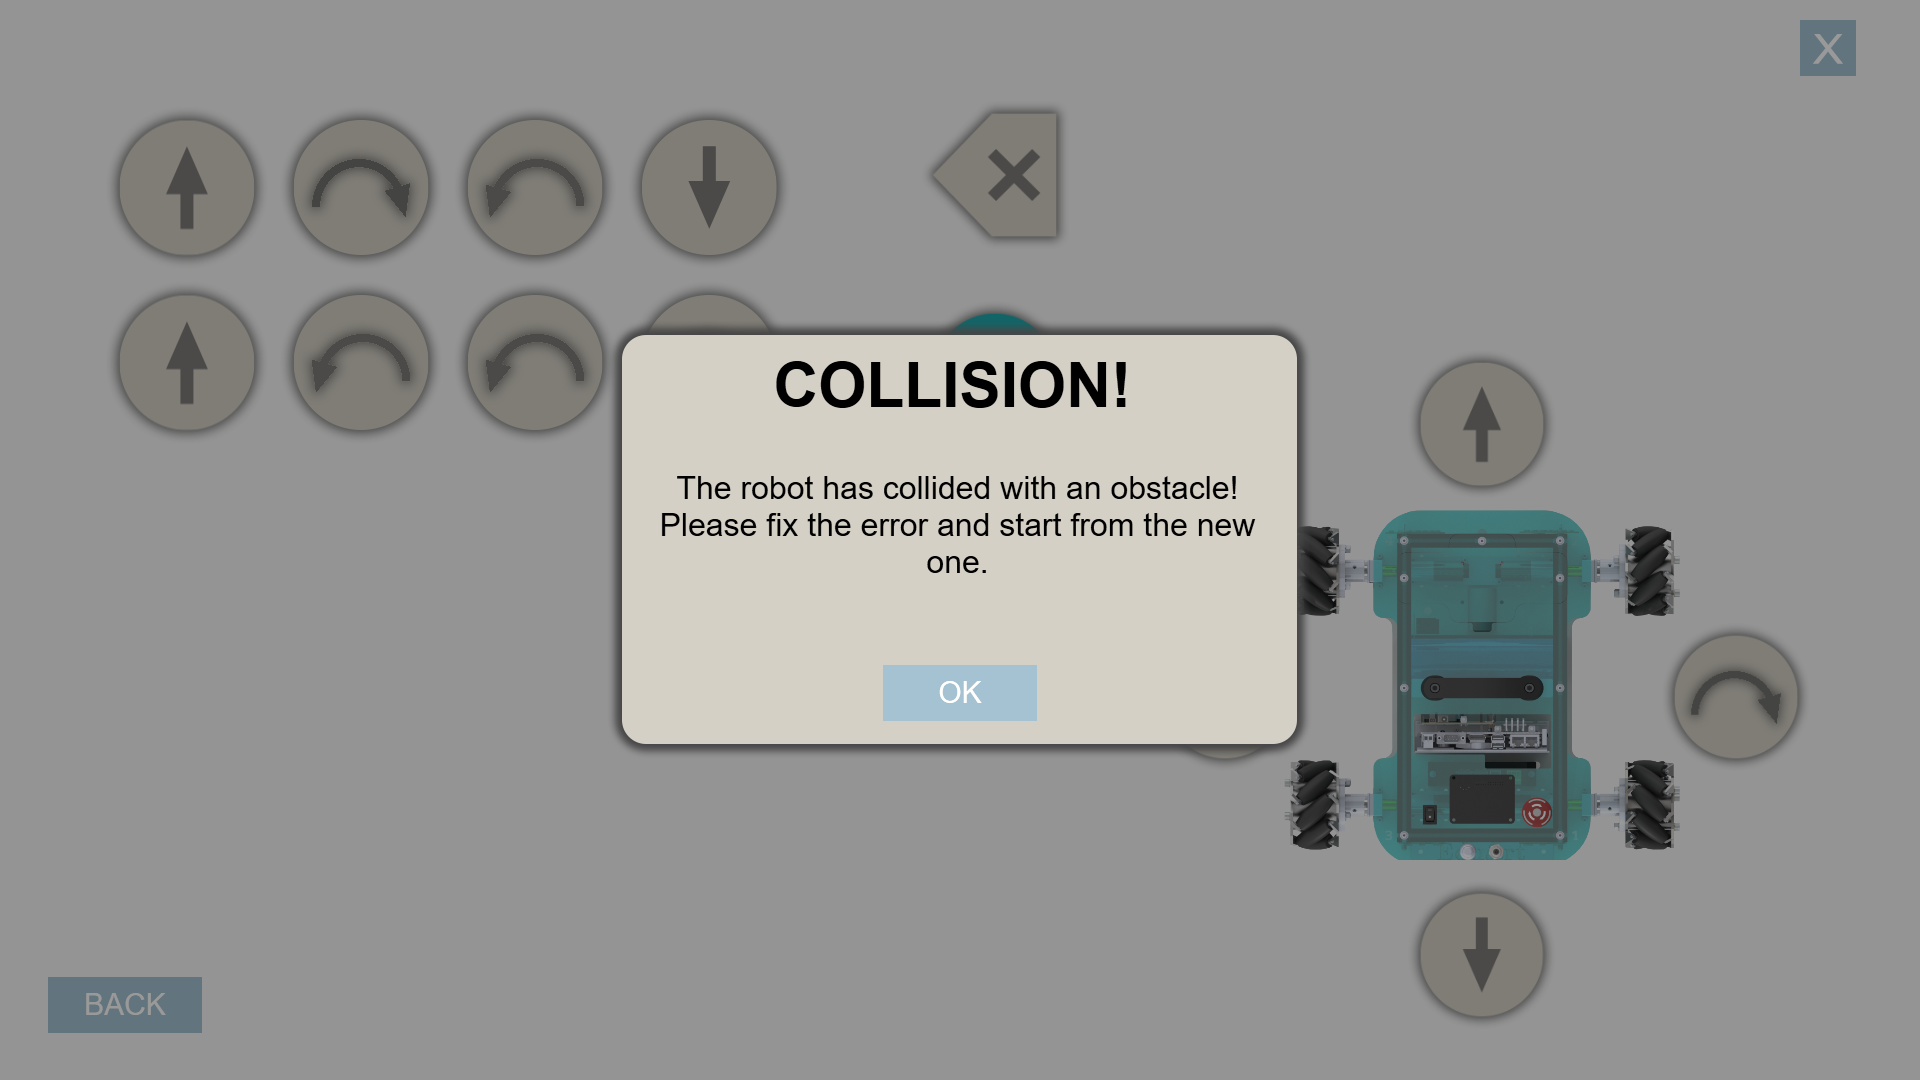
\includegraphics[width=0.5\linewidth]{Bilder/Tests/kollision_en.PNG}}%
  \qquad
  \subfloat[][]{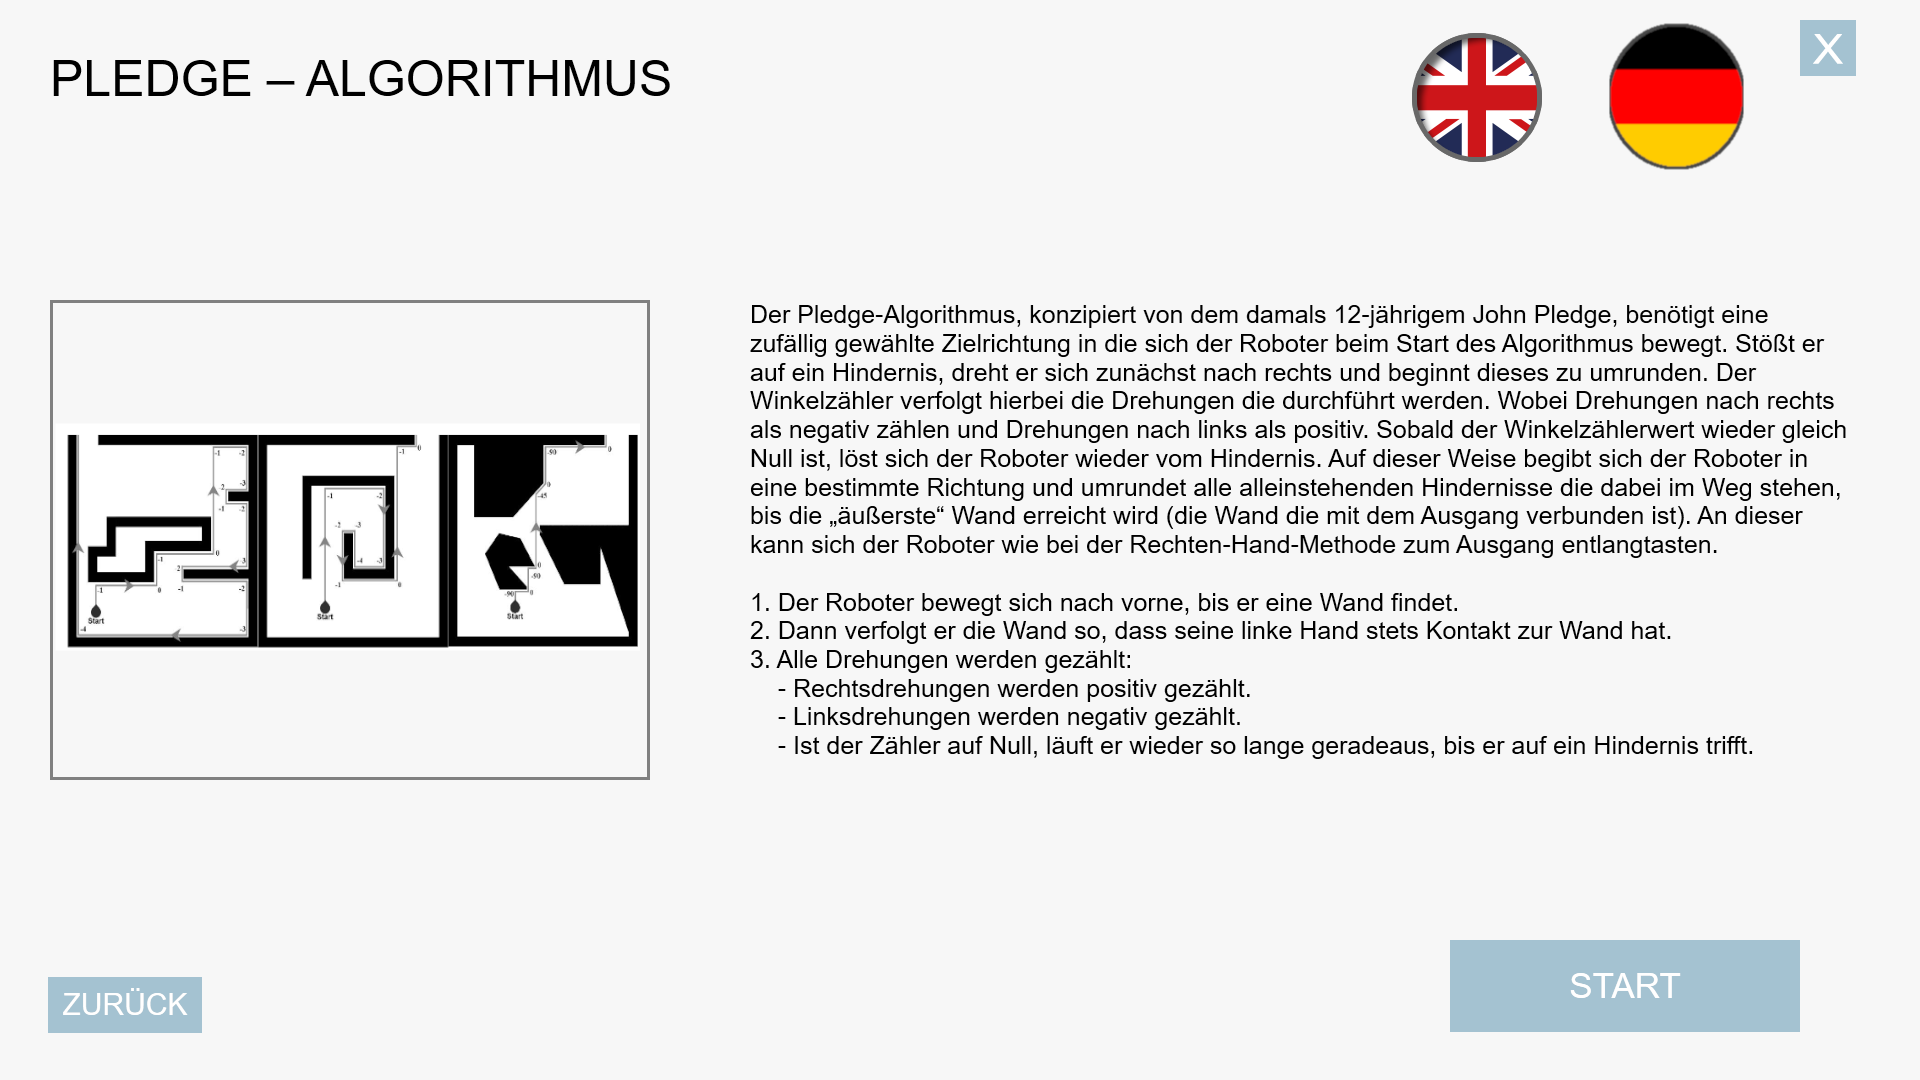
\includegraphics[width=0.5\linewidth]{Bilder/Tests/pledge_de.PNG}}%
  \subfloat[][]{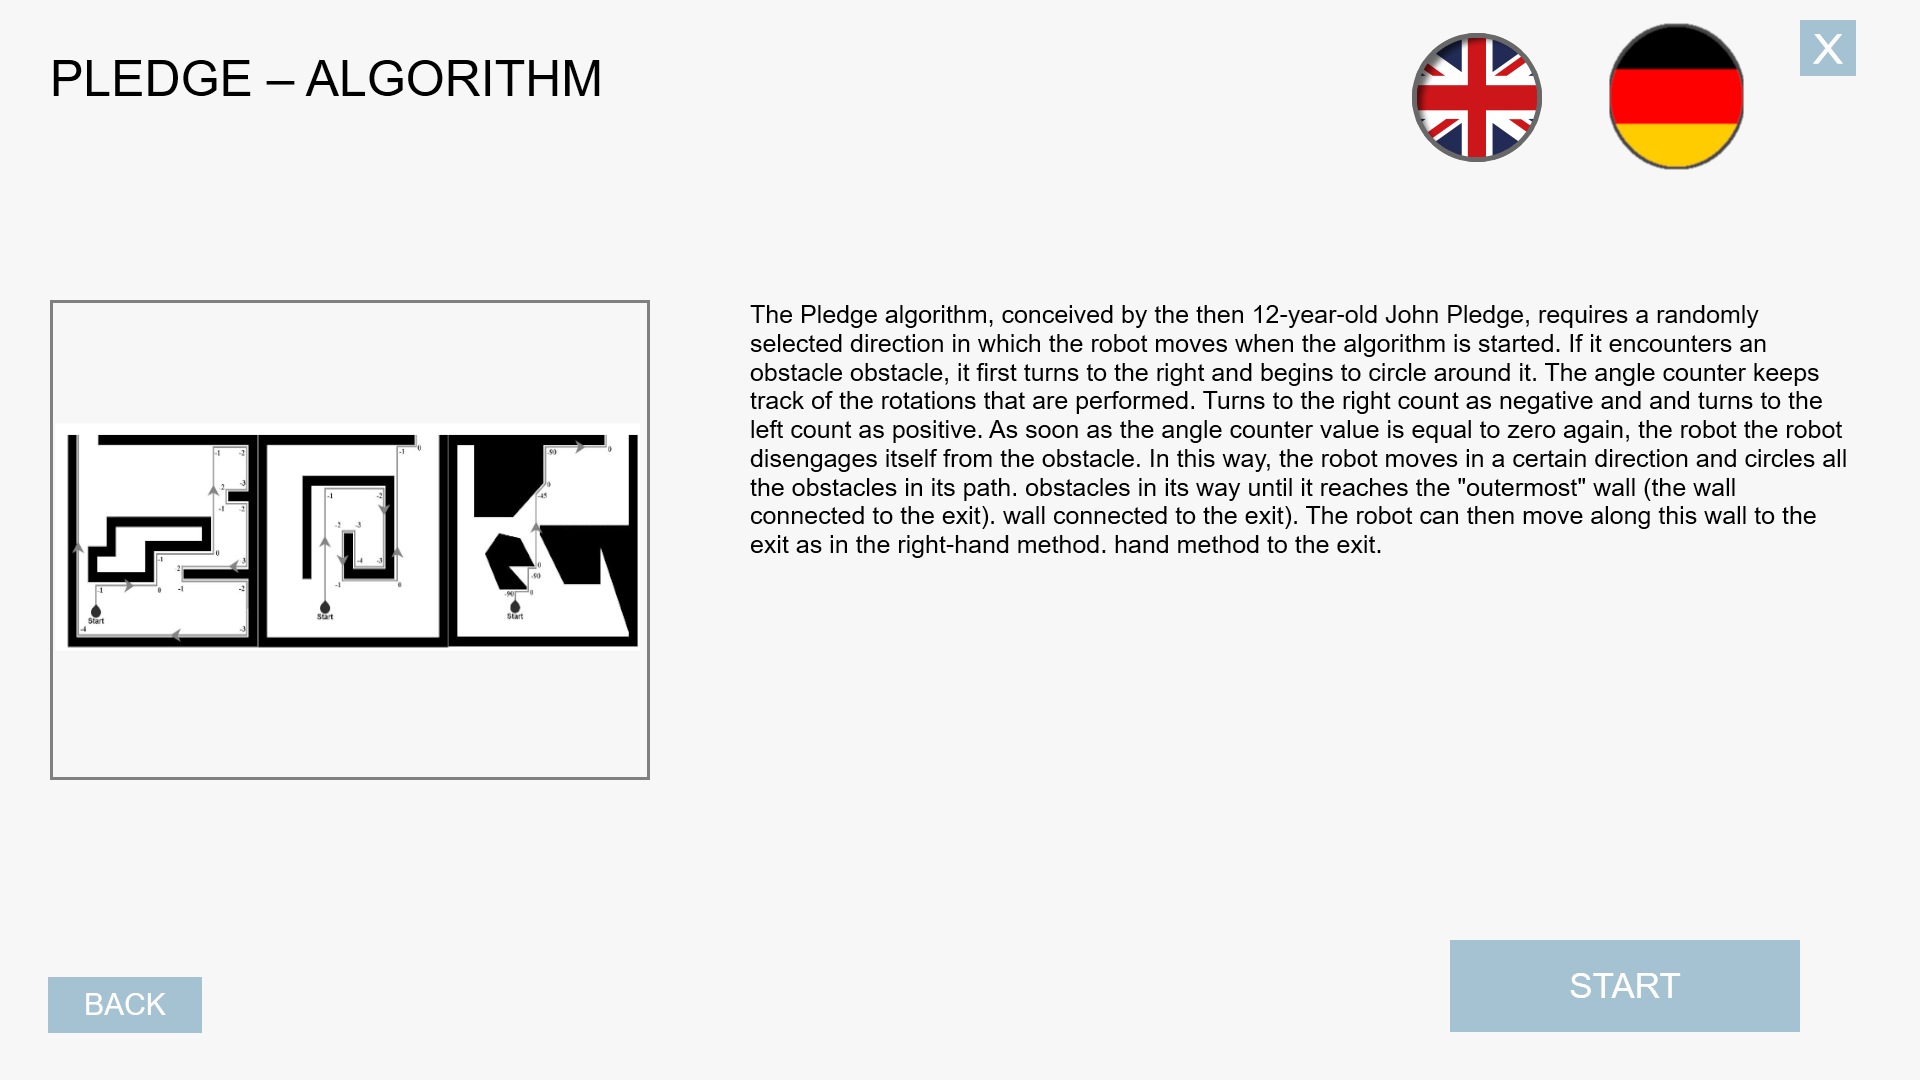
\includegraphics[width=0.5\linewidth]{Bilder/Tests/pledge_en.PNG}}%
  \caption{Test Benutzeroberfläche}
  \label{fig:GUI}
\end{figure}


% \begin{figure}[H]
%  \centering
%  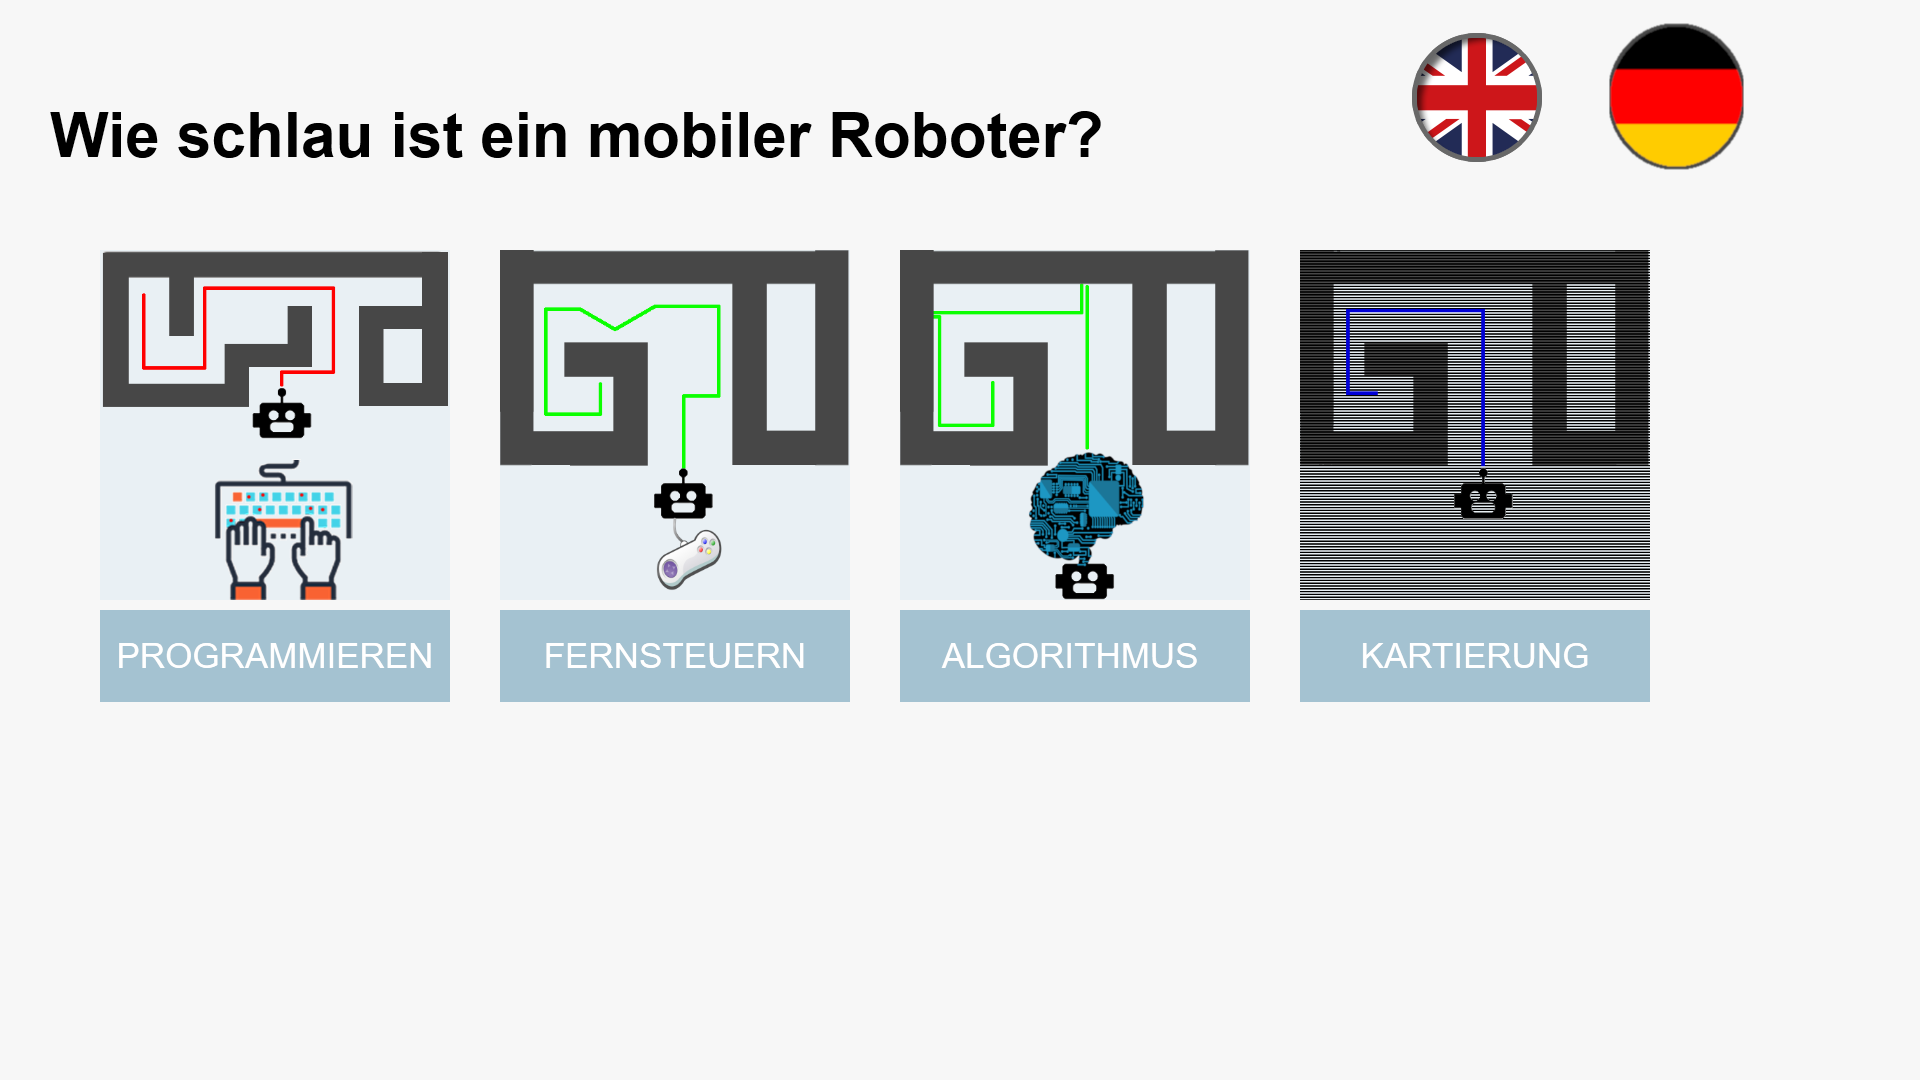
\includegraphics[width=\linewidth]{Bilder/Tests/home_de.PNG}
%  \caption{GUI}
%  \label{fig:GUI}
% \end{figure}

